\label{sec:tcomm}
In addition to the compute to I/O ratio discussed in Section \ref{sec:bound} we define another performance parameter called the compute to communication ratio $t_{\text{comp}}/t_{\text{comm}}$.
In Section \ref{sec:I/O}, we overcame the I/O effect by splitting the trajectory, but scaling remained far from ideal when MPI communication was used (instead of  Global Arrays).
This is because the task remained communication bound (Figure \ref{fig:MPIwithIO-split}), i.e, 
\begin{gather*}
  \frac{t_{\text{comp}}}{t_{\text{comm}}} \ll 1.
\end{gather*}

Figure \ref{fig:tcom_tcomm_effect} shows the relationship of performance with $\overline{\tcomp}/\overline{\tcomm}$ ratio.
When the $\overline{\tcomp}/\overline{\tcomm}$ ratio is higher (Figure \ref{fig:tcomp_tcomm_ratio}), performance is better (Figure \ref{fig:S1_tcomp_tcomm_effect}) even if communication time is larger (Figure \ref{fig:Comm_time_tcomp_tcomm_effect}).
Although, we still observed stragglers due to communication at larger $\overline{\tcomp}/\overline{\tcomm}$ ratios ($70\times$ RMSD and $100\times$ RMSD), their effect on performance remained modest because the overall performance was dominated by the compute load. 
Evidently, if overall performance is dominated by a component such as compute that scales well, then performance problems with components such as communication will be masked and overall acceptable performance can still be achieved (Figures \ref{fig:S1_tcomp_tcomm_effect} and \ref{fig:tcomp_tcomm_ratio}).

Communication is usually not problematic within one node because of the shared memory environment (for less than 24 processes (single compute node on \emph{SDSC Comet}) the scaling is good and $\frac{\tcomp}{\tcomm} \gg 1$ for all RMSD loads) (Figures \ref{fig:S1_tcomp_tcomm_effect} and \ref{fig:tcomp_tcomm_ratio}).
However, beyond a single compute node, scaling appears to get better as the $\overline{\tcomp}/\overline{\tcomm}$ ratio increases and communication overhead becomes less dominant (Figures \ref{fig:S1_tcomp_tcomm_effect} and \ref{fig:tcomp_tcomm_ratio}, 24-72 cores represent multiple compute nodes on \emph{SDSC Comet}).

\begin{figure}[ht!]
\centering
\begin{subfigure} {.33\textwidth}
  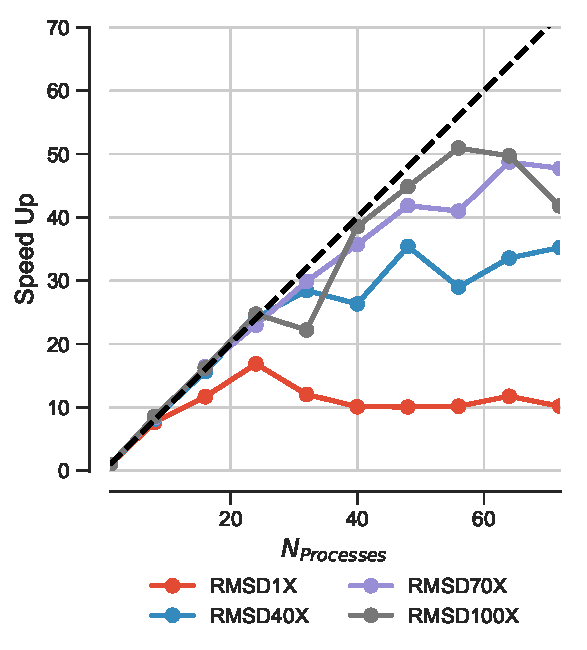
\includegraphics[width=\linewidth]{figures/Compute_to_IO_ratio_on_performance_2d_v17.pdf}
  \caption{Speed-Up}
  \label{fig:S1_tcomp_tcomm_effect}
\end{subfigure}
\hfill
\begin{subfigure}{.3\textwidth}
  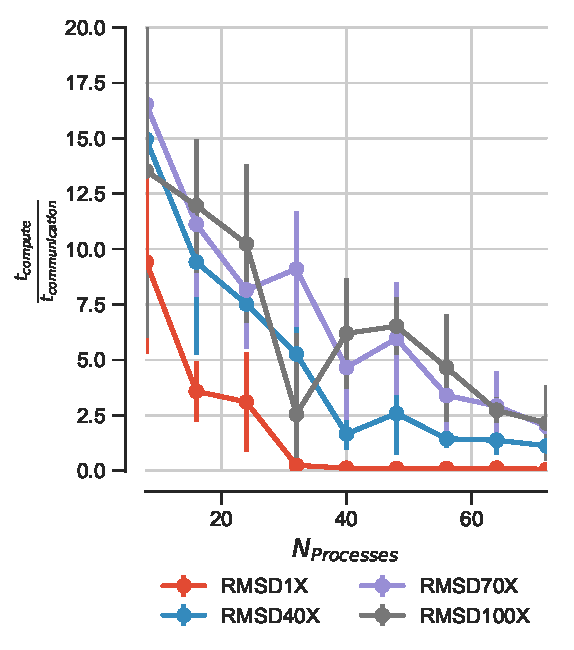
\includegraphics[width=\linewidth]{figures/Compute_to_comm_ratio_on_performance_v17.pdf}
  \captionsetup{format=hang}
\caption{Compute to communication ratio}
\label{fig:tcomp_tcomm_ratio}
\end{subfigure}
\hfill
\begin{subfigure}{.33\textwidth}
  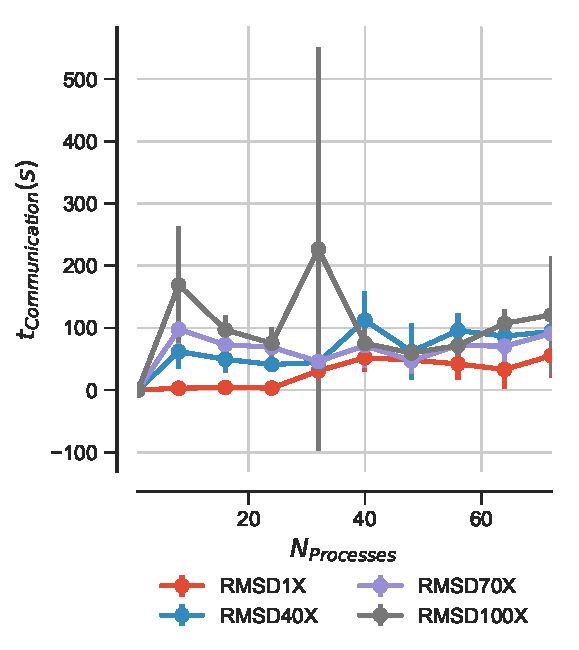
\includegraphics[width=\linewidth]{figures/comm_comparison_different_RMSD_overload.pdf}
  \caption{Communication time}
  \label{fig:Comm_time_tcomp_tcomm_effect}
\end{subfigure}
\caption{(a) Change in compute to communication ratio with number of processes for different RMSD workload on SDSC Comet. 
(b) Comparison of communication time for different RMSD workload on SDSC Comet.
Five repeats were performed to collect statistics and error bars show standard deviation with respect to mean.}
\label{fig:tcom_tcomm_effect}
\end{figure}

%%% Local Variables:
%%% mode: latex
%%% TeX-master: t
%%% End:
